\documentclass[a4paper,12pt,twocolumn]{article}

% Packages
\usepackage{graphicx}
\usepackage{caption} % more customisation options for captions, used for fontsize in figures.
\usepackage{amsmath} % more function within maths environments, namely \text{}

% Making cites superscript
\usepackage[sorting=none]{biblatex}
\DeclareCiteCommand{\supercite}[\mkbibsuperscript]
{\iffieldundef{prenote}
	{}
	{\BibliographyWarning{Ignoring prenote argument}}%
	\iffieldundef{postnote}
	{}
	{\BibliographyWarning{Ignoring postnote argument}}}
{\usebibmacro{citeindex}%
	\bibopenbracket\usebibmacro{cite}\bibclosebracket}
{\supercitedelim}
{}
\let\cite=\supercite

% Adding the bibliography file
\addbibresource{references.bib}

\begin{document}
	
	\begin{titlepage}
		\begin{center}
			
			\thispagestyle{empty}
			
			\Huge{
				\textbf{UCD School Of Physics}
			}
			
			\vspace{1cm}	
			
			
\includegraphics[scale=0.08]{UCDLogo.png}
			
			\vspace{1cm}
			
			\large{
				\textbf{PHYC30170 Physics with Astronomy and Space Science Lab 1; \\
					CCDs and Spectroscopy \\
					\vspace{1cm}
					18/10/2022 \\
					\vspace{1cm}
					Daragh Hollman}
			} \\
			
		\end{center}
	\end{titlepage}
	
	\twocolumn[
	\begin{@twocolumnfalse}
		\begin{abstract}
			The aim of this experiment was to calibrate a CCD for spectroscopy and determine the resolution of the spectrograph. This was done by comparing the emission spectrum of a mercury arc lap to reference values. The gain and readnoise were calculated to be $(1.58 \pm 0.74)\times 10^{-3}$ and $(36.5 \pm 17.3) \,\text{electrons}$ respectively. The resolution of the spectrograph was also calculated for four different wavelengths: 419.1 nm, 496.7 nm, 514.5 nm and 571.4 nm which had resolutions of $207\pm17$, $305\pm35$, $285\pm39$ and $301\pm45$ respectively. The resolution was determined to have a proportional dependence on frequency and an inverse dependence on the slit width.
		\end{abstract}
	\end{@twocolumnfalse}
	]
	
	\section{Introduction}
		A CCD or Charge Coupled Device is an array of light sensitive elements which collect electrons based on the amount of incident light\cite{specInst}. CCDs are frequently used in astronomical imaging due to their high quantum efficiency, large pixel count, cost, and their low noise. CCDs are often used as part of a spectrograph, as in this experiment, to obtain a measurement of flux as a function of wavelength\cite{manual}.
	
	\section{Theory}
		\subsection{Diffraction}
			A diffraction grating is used to split incident light into its separate wavelengths. As a diffraction grating is an array of very narrow and evenly spaced slits, the diffraction pattern from each slit interferes such that the light disperses by a angle $\theta$ as described by equation \ref{eq:diffraction}\cite{universityPhysics}.
			\begin{equation}
				n \lambda = d sin\theta
				\label{eq:diffraction}
			\end{equation} where $d$ is the spacing between the slits, 	$\lambda$ is the wavelength of the incident light, $\theta$ is the angle which the light is diffracted by and $n$ is a positive integer. This process is the primary element of a spectrograph as each discrete wavelength of the light source will be diffracted at a different angle.\\
		
		\subsection{The Spectrograph}	
			A spectrograph is an instrument used to measure incoming light and record its spectrum\cite{atnf}. It splits the incoming light based on its wavelength through diffraction. There are five key components to a spectrograph: telescope, slit, collimator, diffraction grating and detector, as shown in figure \ref{fig:spectrograph}. The telescope focuses the incident light on the slit which only allows a small (ideally 1D) slice of the target through\cite{manual}. The light diverges after the slit and so a collimator is used to make the rays parallel again to ensure that all parts of the light hit the grating at the same angle of incidence. The light then hits the grating and is diffracted at an angle according to its wavelength which the detector picks up.
		
			\begin{figure}
				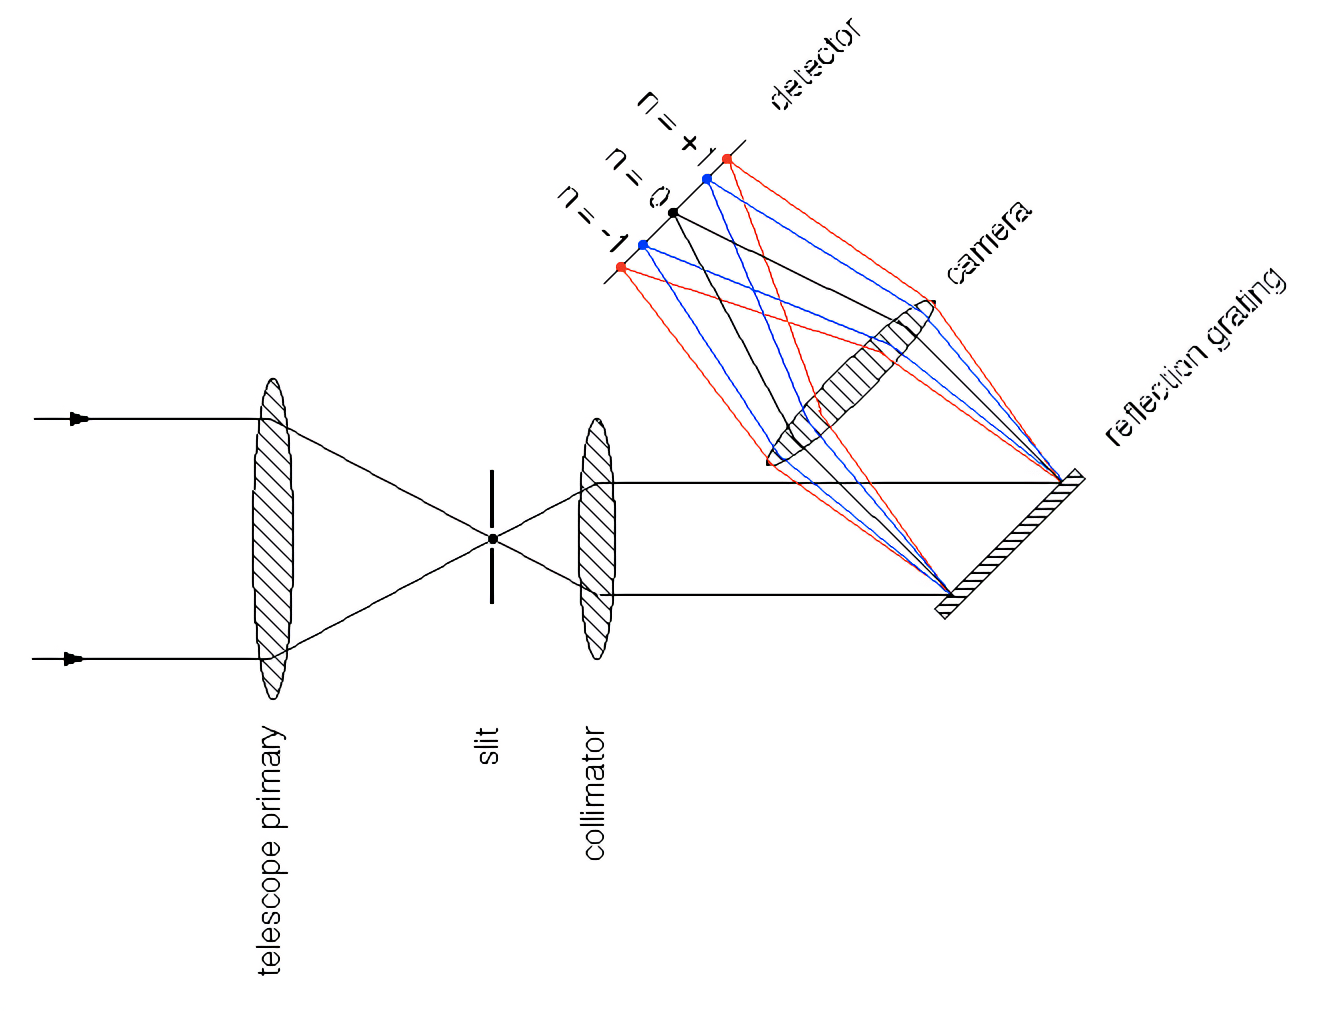
\includegraphics[width=\columnwidth]{spectrograph_refl-transformed.png}
				\captionsetup{font=scriptsize}
				\caption{Diagram of a sample spectrograph setup\cite{vik}. The primary lens focuses the incident light through a slit. The collimator makes the rays parallel as they diffract off of the reflection grating. A last lens focuses the rays on the detector.}
				\label{fig:spectrograph}
			\end{figure}
		
		\subsection{Arc Lamp}
			To calibrate the spectrograph, a spectrum with known emission lines is necessary. To ensure this, an arc lamp is used. An arc lamp produces light by creating an electrical arc of very high current between two conducting electrodes\cite{maglab}. This arc travels through a vapour (mercury or sodium in this instance) which produces light. The lamp emits light at discrete wavelengths depending on what substance is used.
			
		\subsection{Data Reduction}
			When taking measurements with the spectrograph there exists a level of background noise which must be accounted for to ensure accurate measurements. Removing this noise is known as data reduction\cite{manual}. This noise comes from many things including readout electronics, thermal emissions, and non-uniformities in the detector\cite{astropy}. To reduce these noises, images known as flats and biases are used. Flats, or flat field images, are uniformly illuminated images to correct for non-uniformities in the detector. Biases are images taken with ideally a zero second exposure time. They contain no light and hence provide a constant offset which can be subtracted from all further images.\\
			
		Therefore, in this experiment to calibrate to CCD, we will first take flat and bias images to determine the readnoise and gain and will then take images of arc lamps of substances with known emission spectra to calibrate the CCD and determine its resolution.
	
	\section{Methodology}
		\subsection{Apparatus}
			\begin{figure}
				\includegraphics[width=\columnwidth]{ccdDiagram.png}
				\captionsetup{font=scriptsize}
				\caption{Diagram showing the physical setup of the experiment\cite{manual}. The apparatus follows the diagram in figure \ref{fig:spectrograph} with the addition of a neutral density filter to reduce the intensity of the light at all wavelengths. The focal lengths of the focussing lens, collimator and demagnifying lens were 100mm, 225mm and 50mm respectively.}
				\label{fig:apparatus}
			\end{figure}
		
			The apparatus was setup as shown in figure \ref{fig:apparatus} and all lenses were moved to be approximately at the right position to focus the light. The Atik 314L+ CCD was used for this experiment. The CCD was kept below -5.5$^{\circ}$C to negate the effect of thermal noise on the detector.
	
		\subsection{Determining Gain and Readnoise}
			To calibrate the CCD, the gain and readnoise need to be calculated. These quantities were calculated using two flats and two biases as follows in equations \ref{eq:gain} and \ref{eq:readnoise}\cite{manual}.
			
			\begin{equation}
				\text{gain} = \frac{(\overline{\text{flat}_1} + \overline{\text{flat}_2}) - (\overline{\text{bias}_1} + \overline{\text{bias}_1})}{\sigma_{flatdif}^2 - \sigma_{biasdif}^2}
				\label{eq:gain}
			\end{equation}
			\begin{equation}
				\text{readnoise} = \text{gain} \times \frac{\sigma_{biasdif}}{\sqrt{2}}
				\label{eq:readnoise}
			\end{equation} where $\overline{\text{flat}_n}$ are the mean pixel value of the nth flat frame and $\overline{\text{bias}_n}$ the same for the nth bias frame, while $\sigma_{flatdif}$ and $\sigma_{biasdif}$ are the standard deviations of these pixel values. 30 bias frames were taken at an exposure of 0.001 seconds, the lowest possible exposure with the given software and apparatus, and 15 flat frames were taken at 	0.1 seconds.\\
			
			For each pair of bias frames and flat frames, the gain and readnoise were calculated. To increase precision, the calculations for gain and readnoise were repeated for 7 pairs of flats and 15 pairs of biases and then averaged to get average and uncertainty values.
		
		\subsection{Wavelength Calibration}
			To calibrate the spectrograph with respect to wavelength, a mercury arc lamp was used. As the wavelength of the emission lines of the mercury lamp were known, (see figure \ref{fig:mercury}), this spectrum could be used to identify the lines in the detection and hence a wavelength could be assigned to each x value of the frame. A frame of the mercury arc lamp was then captured. Based off of this image the lenses were adjusted to ensure the emission lines were as sharp as possible.\\
			
			\begin{figure}
				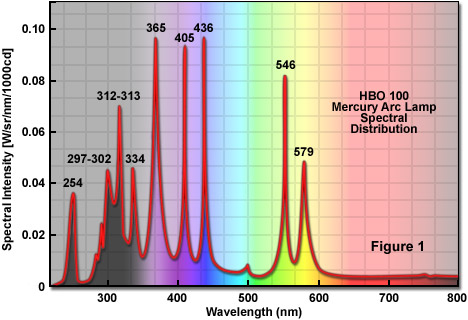
\includegraphics[width=\columnwidth]{mercurySpectrum.jpg}
				\captionsetup{font=scriptsize}
				\caption{The emission spectrum of a mercury arc lamp shown by ZEISS\cite{zeiss}. As the wavelength of each emission line is known, they can be used to calibrate the spectrograph.}
				\label{fig:mercury}
			\end{figure}
			
			A 1D slice at y=800, as shown in figure \ref{fig:Hg}, was taken to observe the counts against the x axis. From this slice, the wavelength of each peak was identified based on the reference spectrum and its x coordinate was plotted against this wavelength. From these points, a line of best fit was produced which could be used to calibrate the CCD. For each x coordinate, a corresponding wavelength could be found based on this fitted line.
			
			\begin{figure}
				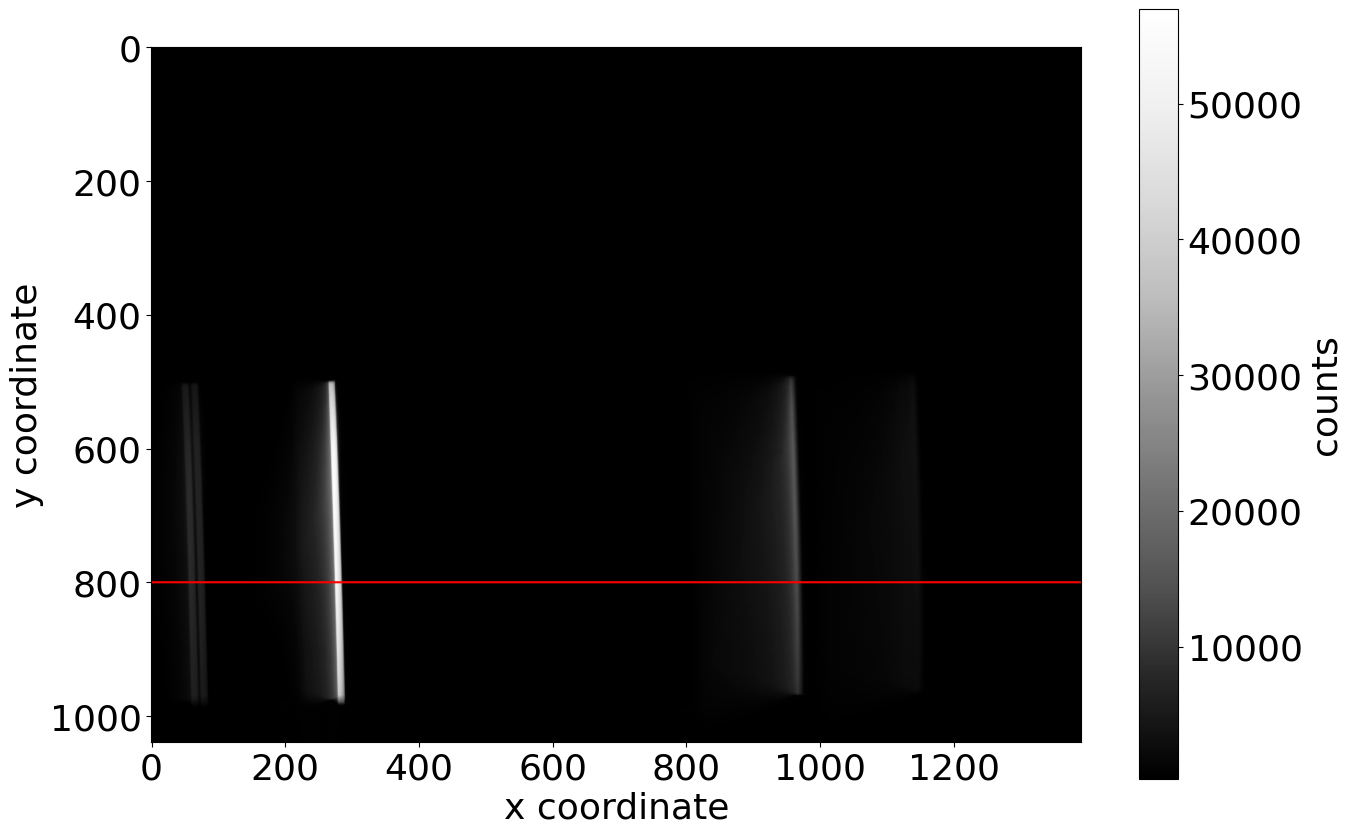
\includegraphics[width=\columnwidth]{mercuryEmission.png}
				\captionsetup{font=scriptsize}
				\caption{The measured emission spectrum of the mercury arc lamp, a 1D slice at y=800 is marked in red and taken as a 1D slice to observe the spectrum.}
				\label{fig:Hg}
			\end{figure}
		
		\subsection{Determining the Resolution of the Spectrograph}
			The resolution of the spectrograph was determined by measurements on a frame taken of a sodium arc lamp. The frame was captured and, as in the case of the mercury frame, a spectrum of counts against the x axis was produced. Using the results of the calibration in the previous section, these x coordinates were transformed such that a spectrum of counts against wavelength was created. The resolution of the spectrograph is defined in equation \ref{eq:resolution}\cite{manual}.
			
			\begin{equation}
				\text{resolution} = \frac{\lambda}{\Delta \lambda}
				\label{eq:resolution}
			\end{equation} where $\lambda$ is the wavelength and $\Delta \lambda$ is the FWHM (full-width half-maximum) of the peak. A gaussian distribution was fitted to each peak of this spectrum and the FWHM of each gaussian was measured, hence determining the resolution. This was repeated for all peaks on the spectrum to determine the dependence of the resolution on the wavelength.
	
	\section{Results and Analysis}
		
		\subsection{Calibration of the Spectrograph}
		The gain was calculated to be $(1.58 \pm 0.74)\times 10^{-3}$ and readnoise was calculated to be $(36.5 \pm 17.3) \,\text{electrons}$. The uncertainties on these measurements was taken as the standard deviation of the list of gains and readnoises.\\
		
		The measured 1D slice of the mercury arc lamp was plotted in figure \ref{fig:HgSpectrum}. The red vertical lines mark the estimated x coordinate of each peak. The uncertainty of each peak was assumed to be an upper limit 15 pixels either side of the mean. The spectrum was compared to the known spectrum of sodium to create a plot with the x coordinate of each peak against the wavelength as shown in figure \ref{fig:calibration}. A linear least squares fit was calculated on the data to create a function to transform an input x coordinate to a wavelength.
		
		\begin{figure}
			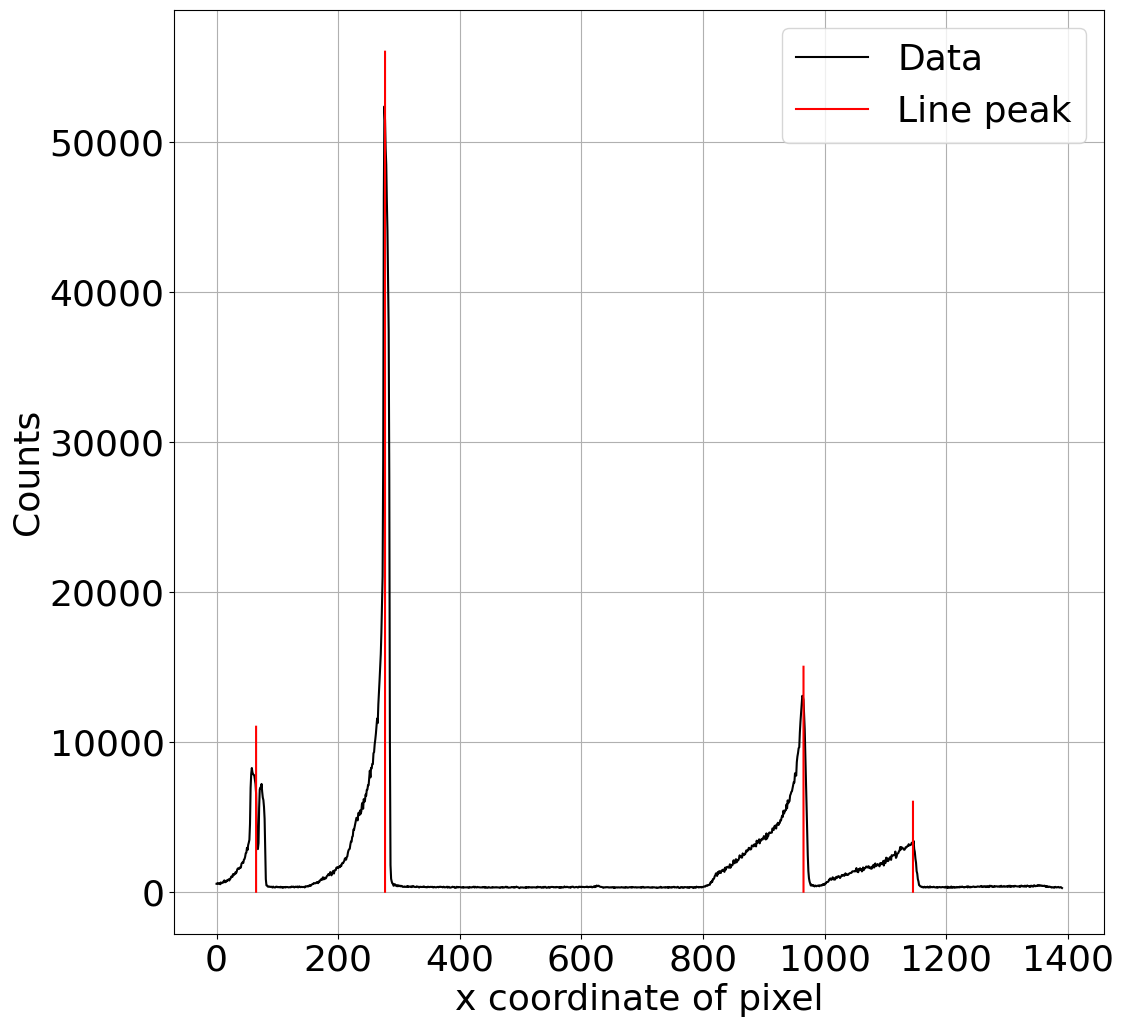
\includegraphics[width=\columnwidth]{HgPeaks.png}
			\captionsetup{font=scriptsize}
			\caption{The 1D slice of the frame shown in figure \ref{fig:Hg}. The red vertical lines mark the estimated x coordinate of each peak with an uncertainty of 15 pixels.}
			\label{fig:HgSpectrum}
		\end{figure}
	
		\begin{figure}
			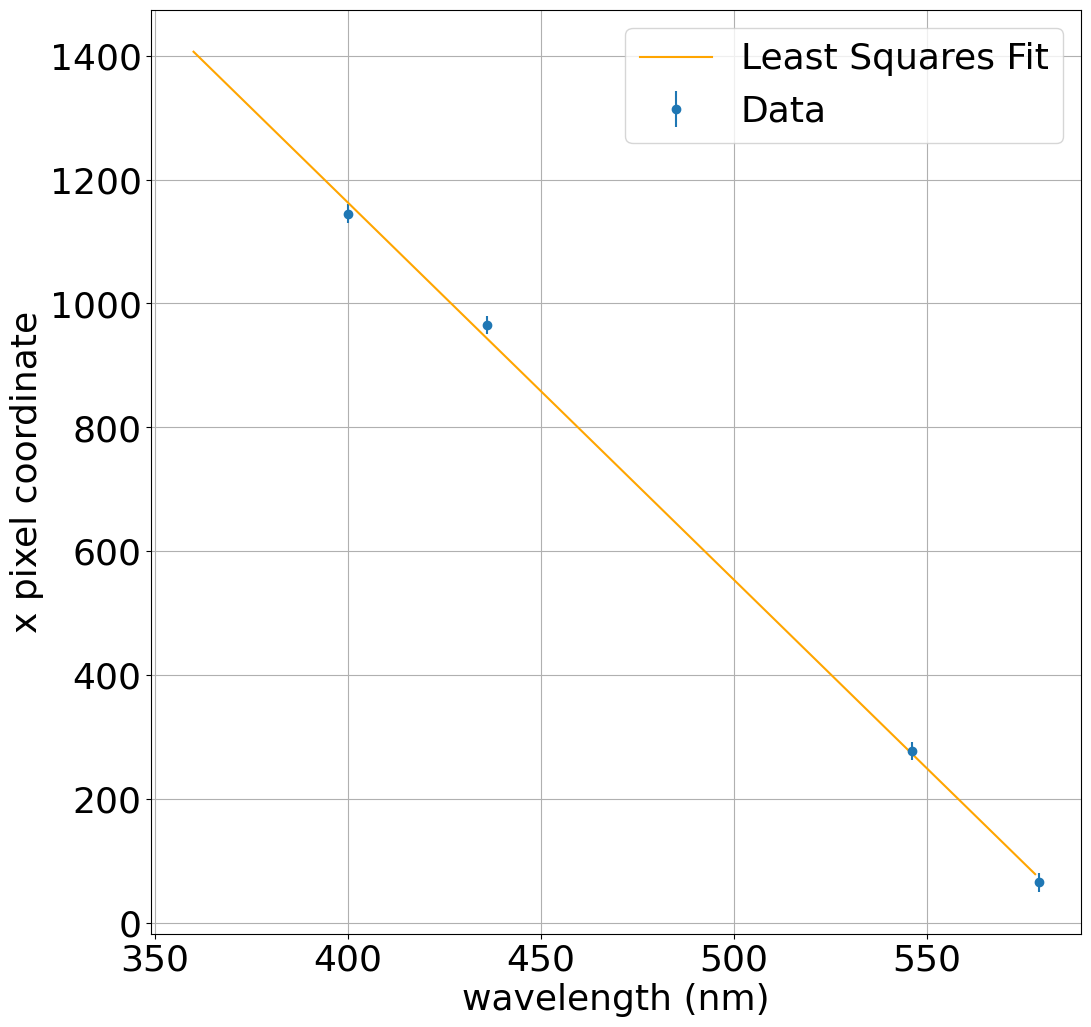
\includegraphics[width=\columnwidth]{calibration.png}
			\captionsetup{font=scriptsize}
			\caption{The calibration plot of the mercury emission peaks. A least squares fit is displayed in orange.}
			\label{fig:calibration}
		\end{figure}
		
		\subsection{Resolution of the Spectrograph}
		A frame of a sodium arc lamp was taken and the calibration function was used to create the spectrum shown in figure \ref{fig:sodiumSpectrum}. Reference data\cite{uci} of a sample sodium emission spectrum was used to ensure the calibration was accurate. The peaks were identified and least squares fitting was used to fit a gaussian distribution to each peak. The FWHM of each gaussian was calculated and using the position of the gaussian, the resolution of the spectrograph was calculated by equation \ref{eq:resolution}. This was repeated for each peak and each value for the resolution was plotted in figure \ref{fig:resolution} against the wavelength of the peak. The resolutions of each peak in order of increasing wavelengths are as follows: $207\pm17$, $305\pm35$, $285\pm39$ and $301\pm45$. A least squares fitting was applied to calculate the wavelength dependence of the resolution. The resolution as a function of wavelength follows the form:
		
		\begin{equation}
			\text{R}(\lambda) = a\lambda + b
		\end{equation} where a is $(0.63 \pm 0.26)\,\text{nm}^{-1}$ and b is $-40 \pm 130$, where the uncertainties on these parameters were calculated by taking the square root of the diagonal elements of the covariance matrix. It is clear that the relative uncertainty on these measurements is large and hence there is not much value to knowing them however, graphically, it is clear that there is a distinct increase in resolution with an increase in wavelength.\\
	
		The sodium arc lamp frame was taken again with the slit width increased to determine if the resolution depended on it. From figure \ref{fig:slitWidth} it is clear to see that the width of each peak is substantially increased for an increase in slit width. It is clear from equation \ref{eq:resolution} that an increase in the width of the peak, and hence FWHM of the gaussian, that the resolution would decrease due to its inverse proportionality.
		
		\begin{figure}
			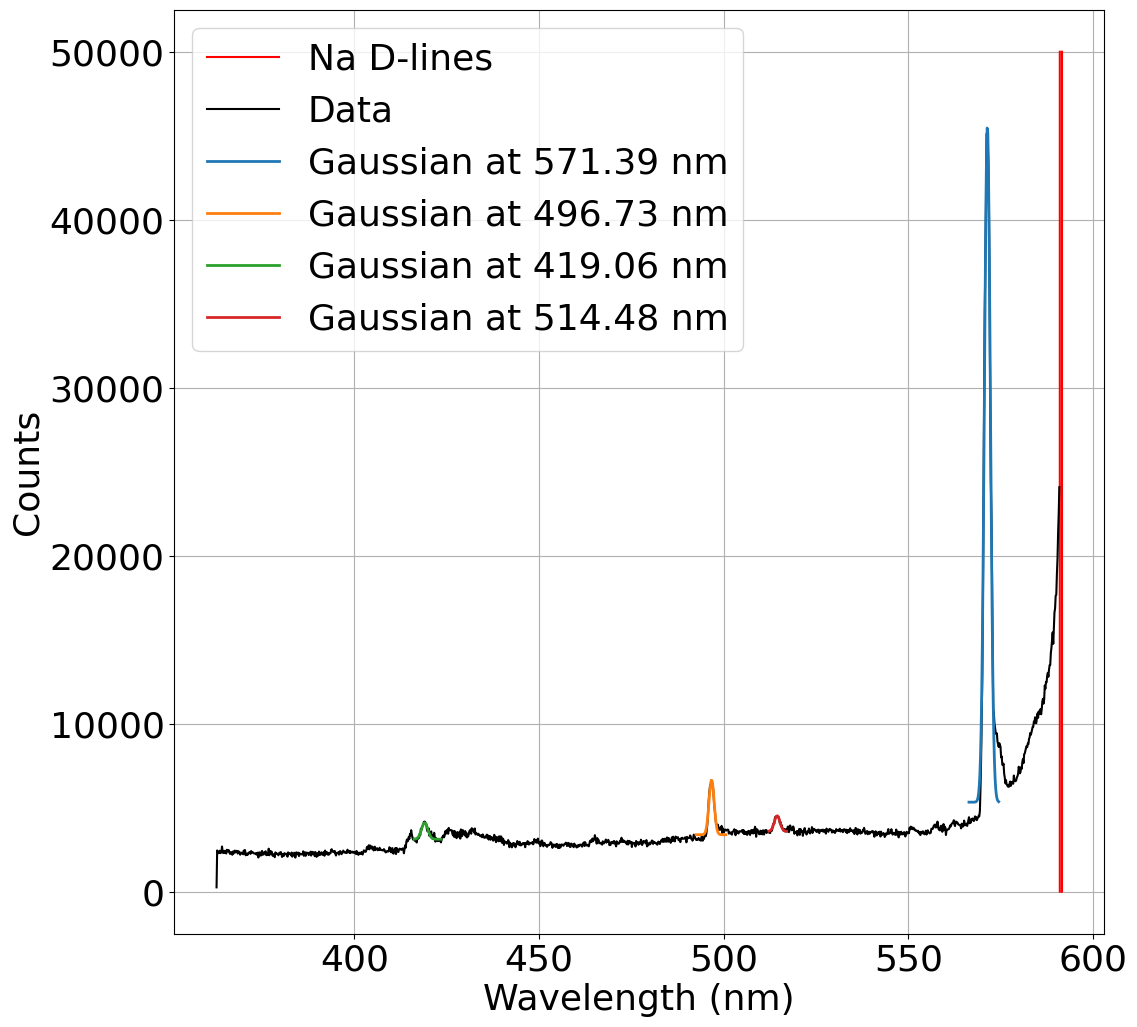
\includegraphics[width=\columnwidth]{sodiumSpectrum.png}
			\captionsetup{font=scriptsize}
			\caption{Spectrum of the sodium arc lamp. A gaussian was fitted to each peak to measure the resolution. The sodium D lines are marked in red, they begin just outside of the view of the detector but their presence is obvious from the quickly increasing data at high wavelengths due to the bleed of light.}
			\label{fig:sodiumSpectrum}
		\end{figure}
	
		\begin{figure}
			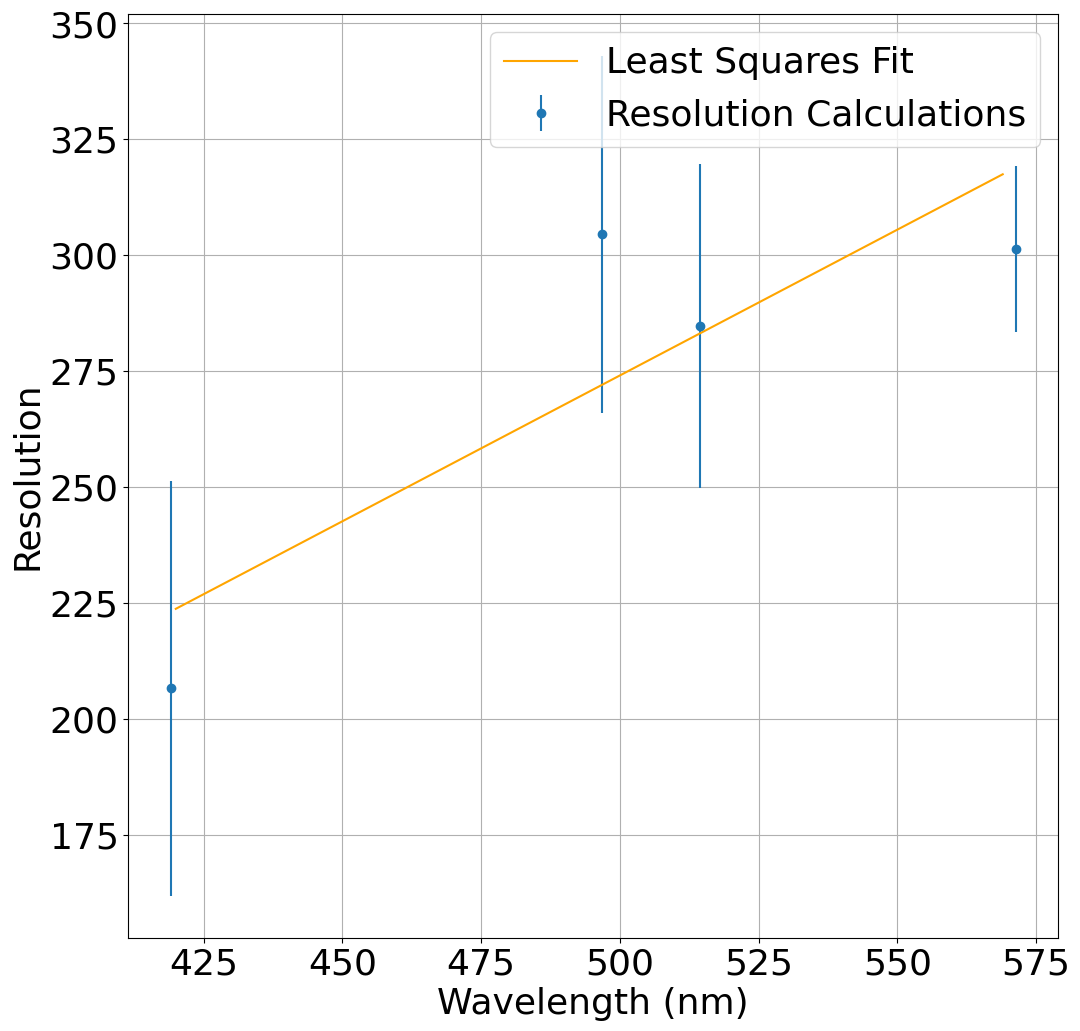
\includegraphics[width=\columnwidth]{resolutions.png}
			\captionsetup{font=scriptsize}
			\caption{The resolution for each peak plotted against its wavelength. Least squares fitting was used to calculate the wavelength dependence of the resolution. The uncertainty on each point was calculated using the propagation of errors method.}
			\label{fig:resolution}
		\end{figure}
	
		\begin{figure}
			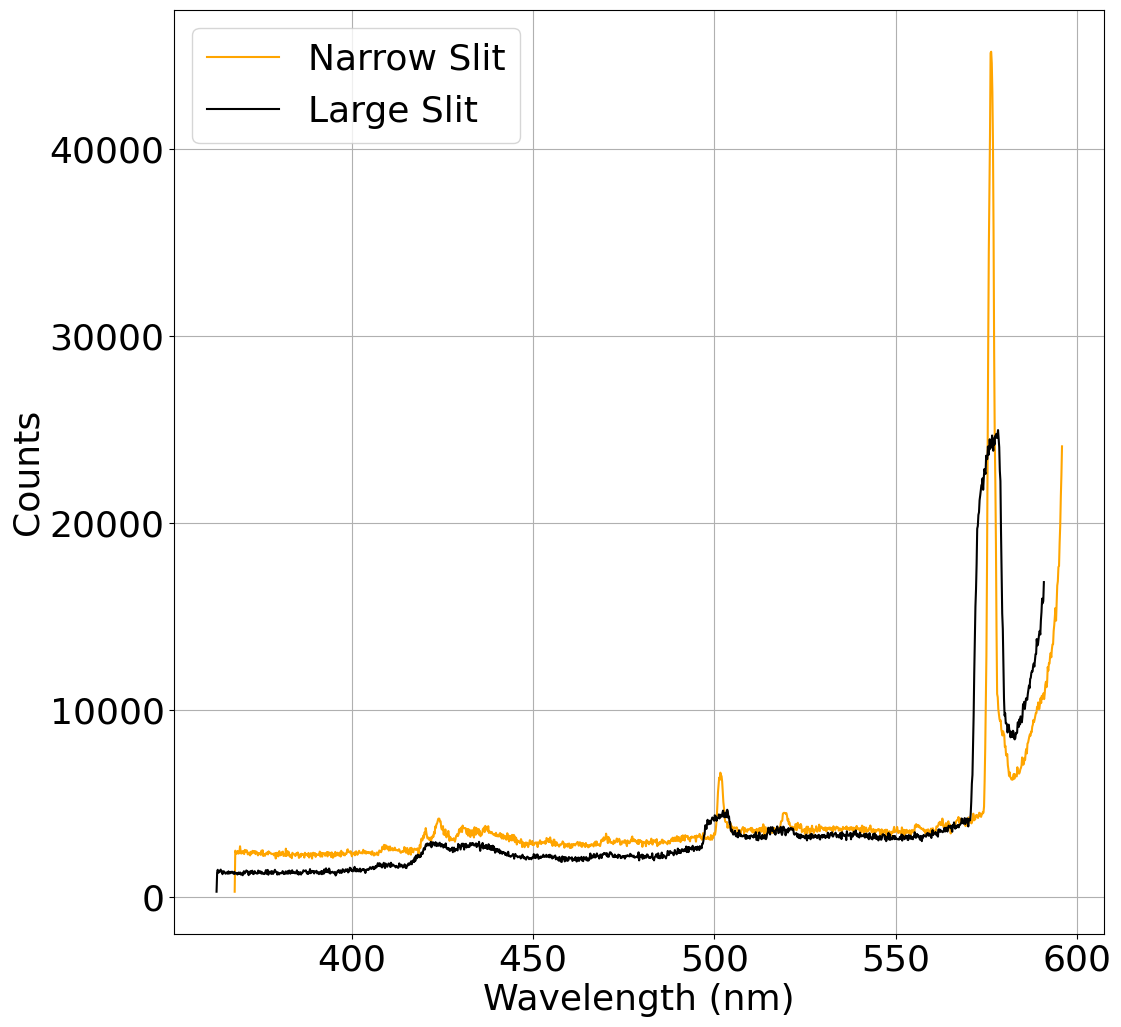
\includegraphics[width=\columnwidth]{slitWidth.png}
			\captionsetup{font=scriptsize}
			\caption{The spectra of the sodium arc lamp with the narrow slit (orange) and the wide slit (black). The exposure had to be adjusted as the larger slit let more light through however it is clear by comparison that the larger slit causes an increase in FWHM.}
			\label{fig:slitWidth}
		\end{figure}
		
	\section{Conclusion}
		In this experiment, the CCD was calibrated by developing a function to transform the x coordinate of pixel to a wavelength. The gain and readnoise were calculated to be $(1.58 \pm 0.74)\times 10^{-3}$ and $(36.5 \pm 17.3) \,\text{electrons}$ respectively. The resolution of the spectrograph was also calculated for four different wavelengths: 419.1 nm, 496.7 nm, 514.5 nm and 571.4 nm which had resolutions of $207\pm17$, $305\pm35$, $285\pm39$ and $301\pm45$ respectively. The resolution was determined to have a proportional dependence on frequency and an inverse dependence on the slit width.
	\newpage
	\printbibliography
	
	\newpage
	\section*{Appendices}
		\subsection{Appendix 1 - Python Code}
		
\end{document}